% !TEX encoding = UTF-8
% !TEX TS-program = pdflatex
% !TEX root = ../thesis.tex

\chapter{State of the art and technology background}
This chapter presents the pre-concepts needed to comprehend this paper's content fully.
As is understandable from the introduction, they are about Self-Sovereign Identity and 
blockchains. In addition, state of the art will be analyzed to see what has already been
done and what can be improved.
% /*//////////////////////////////////////////////////////////////
%                       TECHNOLOGY CONCEPTS
% //////////////////////////////////////////////////////////////*/
\section{Technology concepts}
This section will explain in detail SSI and blockchain technologies.
\subsection{Self-Sovereign Identity concepts}
Here can be read a brief reprise of what has already been saying about Self-Sovereign 
Identity and a description of its main primitives: VCs, VPs, and DIDs.
\subsubsection{Self-Sovereign Identity}
Self-Sovereign Identity is an approach to digital identity that gives individuals 
control over their data. SSI addresses the difficulty of establishing trust in 
interaction and allows people to interact in the digital world with the same freedom 
and ability to trust as they have in the offline world.
\vspace*{0.3cm}\\
To be trusted, a party in an interaction will present credentials to other parties, 
and those parties can verify that the credentials come from an \textbf{issuer} they trust.
This way, the \textbf{verifier}'s trust in the issuer is transferred to the credential 
\textbf{holder} (or \textbf{prover}). This basic structure of SSI with three participants 
is sometimes called the "triangle of trust.", simply because you need an element of trust
among these entities for them to work together.
\vspace*{0.3cm}\\
While this does not mean that there is a legal partnership or understanding between the 
entities involved, it does mean that each of the entities is willing to examine the 
credibility of the other, and this implicit trust is what constitutes this term.
\begin{center}
    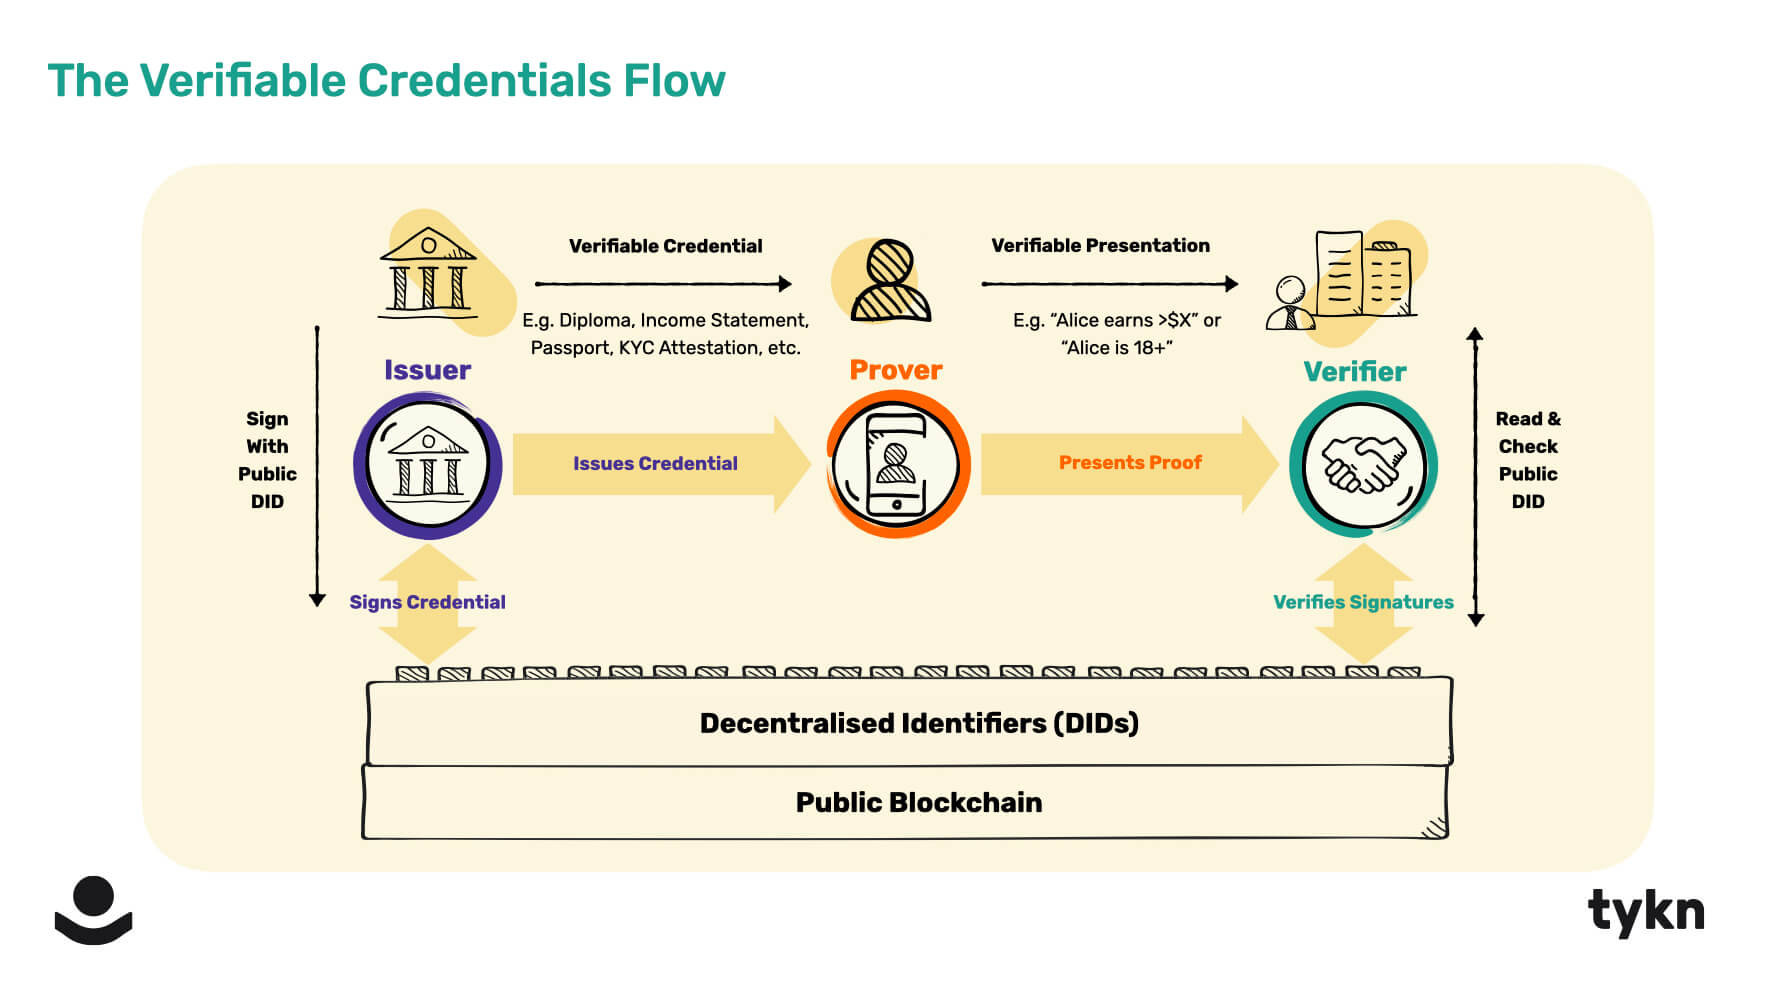
\includegraphics[scale=0.2]{chapter2/triangleTrust2.jpeg}
    \captionof{figure}{The triangle of trust: Prover, Issuer, and Verifier (by Tykn)}
\end{center}
\subsubsection{Verifiable Credential (VC)}
A verifiable credential can represent all of the same information that a physical 
credential represents. The addition of technologies, such as digital signatures, 
makes verifiable credentials more tamper-evident and more trustworthy than their 
physical counterparts.\\
\begin{center}
    \vspace*{-0.5cm}
    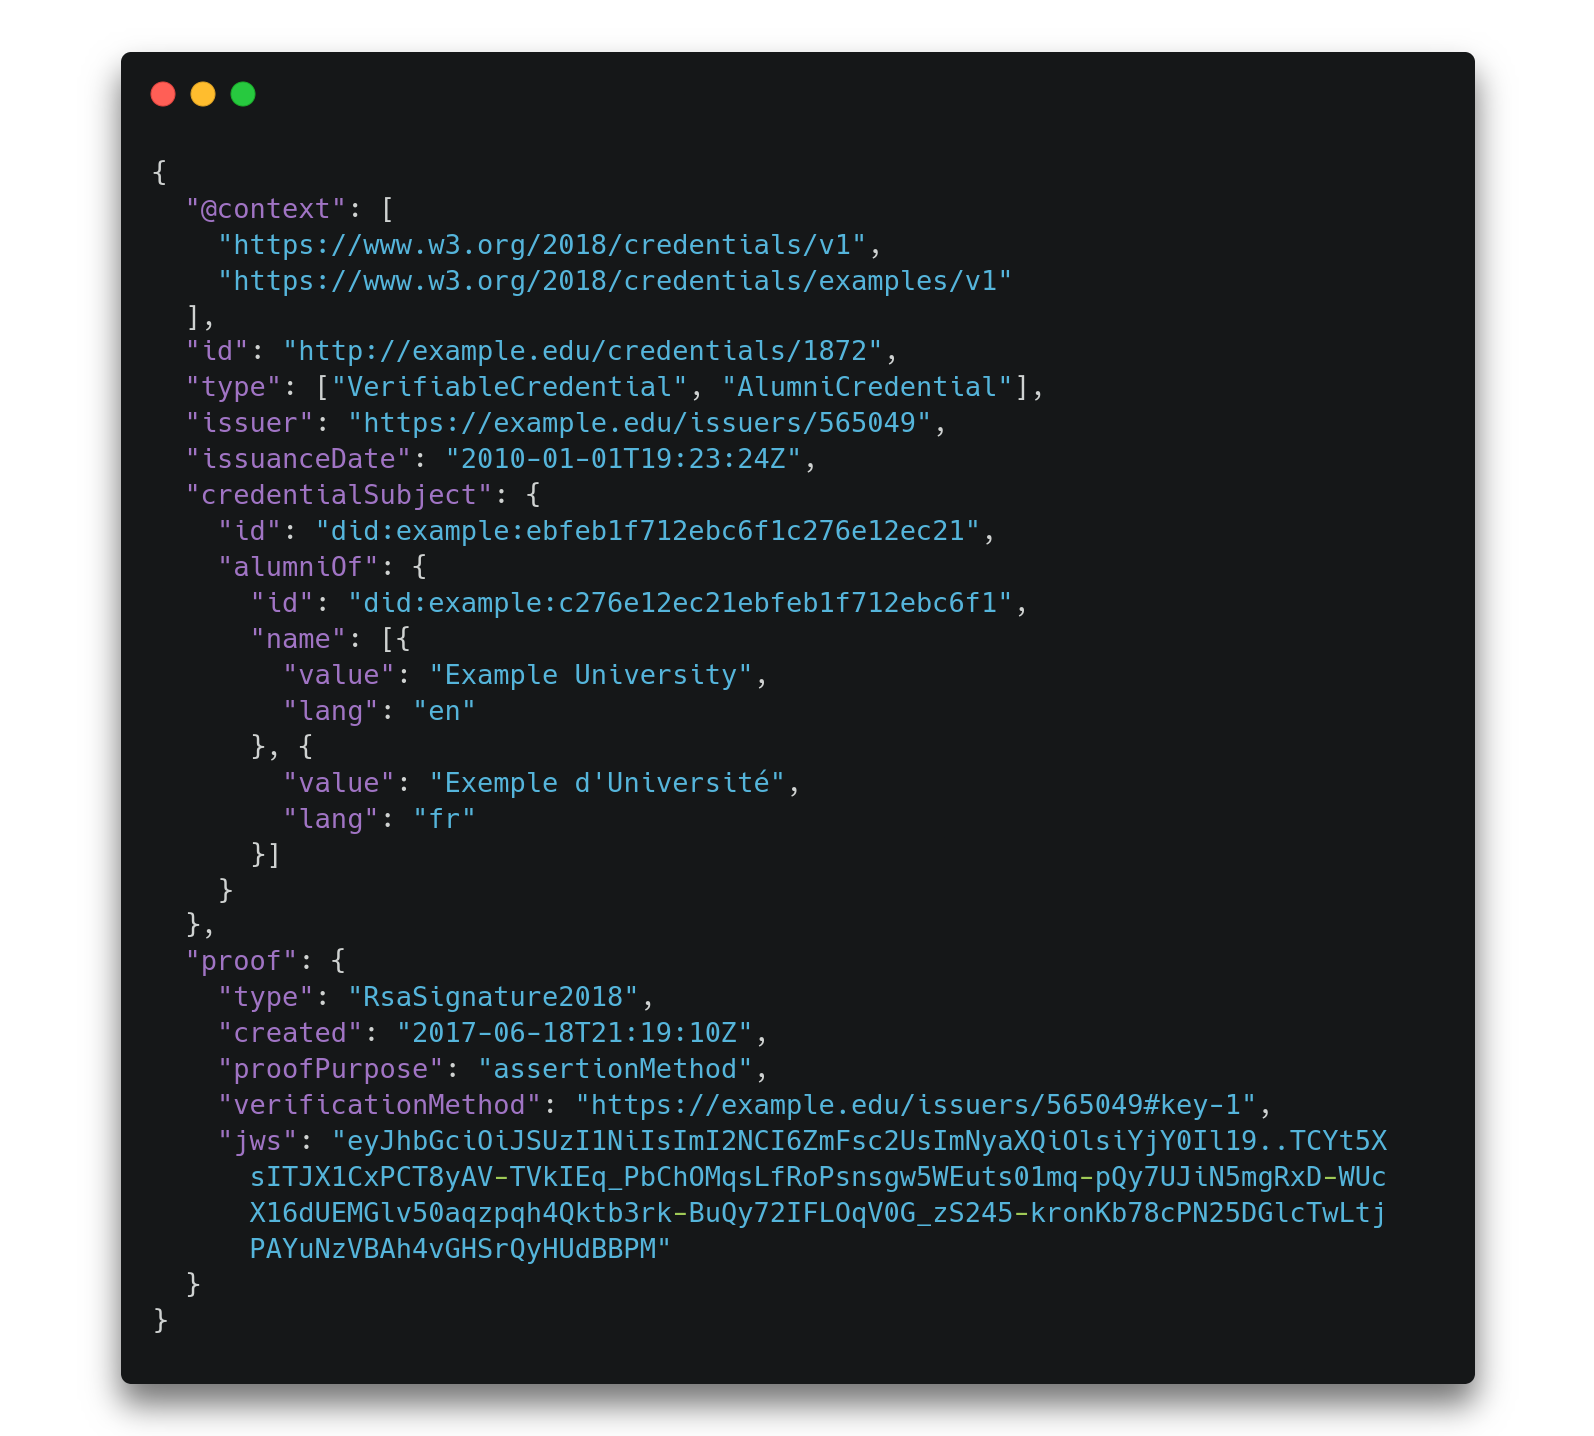
\includegraphics[scale=0.2]{chapter2/exampleVc.png}
    \captionof{figure}{Example of verifiable credential (VC)}
\end{center}
Holders of verifiable credentials can generate verifiable presentations and then share 
these verifiable presentations with verifiers to prove they possess verifiable 
credentials with certain characteristics.\\
Both verifiable credentials and verifiable presentations can be transmitted rapidly, 
making them more convenient than their physical counterparts when trying to establish 
trust at a distance.
The three main components of a VC are:
\begin{enumerate}
    \item \textbf{Metadata}: cryptographically signed by the issuer. It describes the credential
    properties, such as the issuer, the subject, the expiry date and time, a public key 
    to use for verification purposes, the revocation mechanism, and other information;
    \item \textbf{Claims}: a statement made about a subject. Example: “Janice`s date of 
    birth is 01/01/1990.”
    \item \textbf{Proofs}: a proof is data about the identity holder that allows others 
    to verify the source of the data (i.e., the issuer), check that the data belongs to 
    (only) the holder, that the data has not been tampered with, and finally, that the 
    issuer has not revoked the data.
\end{enumerate}

\subsubsection{Verifiable Presentation (VP)}
A verifiable presentation expresses data from one or more verifiable credentials and is 
packaged in such a way that the authorship of the data is verifiable. If verifiable 
credentials are presented directly, they become verifiable presentations. Data formats 
derived from verifiable credentials that are cryptographically verifiable but do not 
themselves contain verifiable credentials might also be verifiable presentations.
\begin{center}
    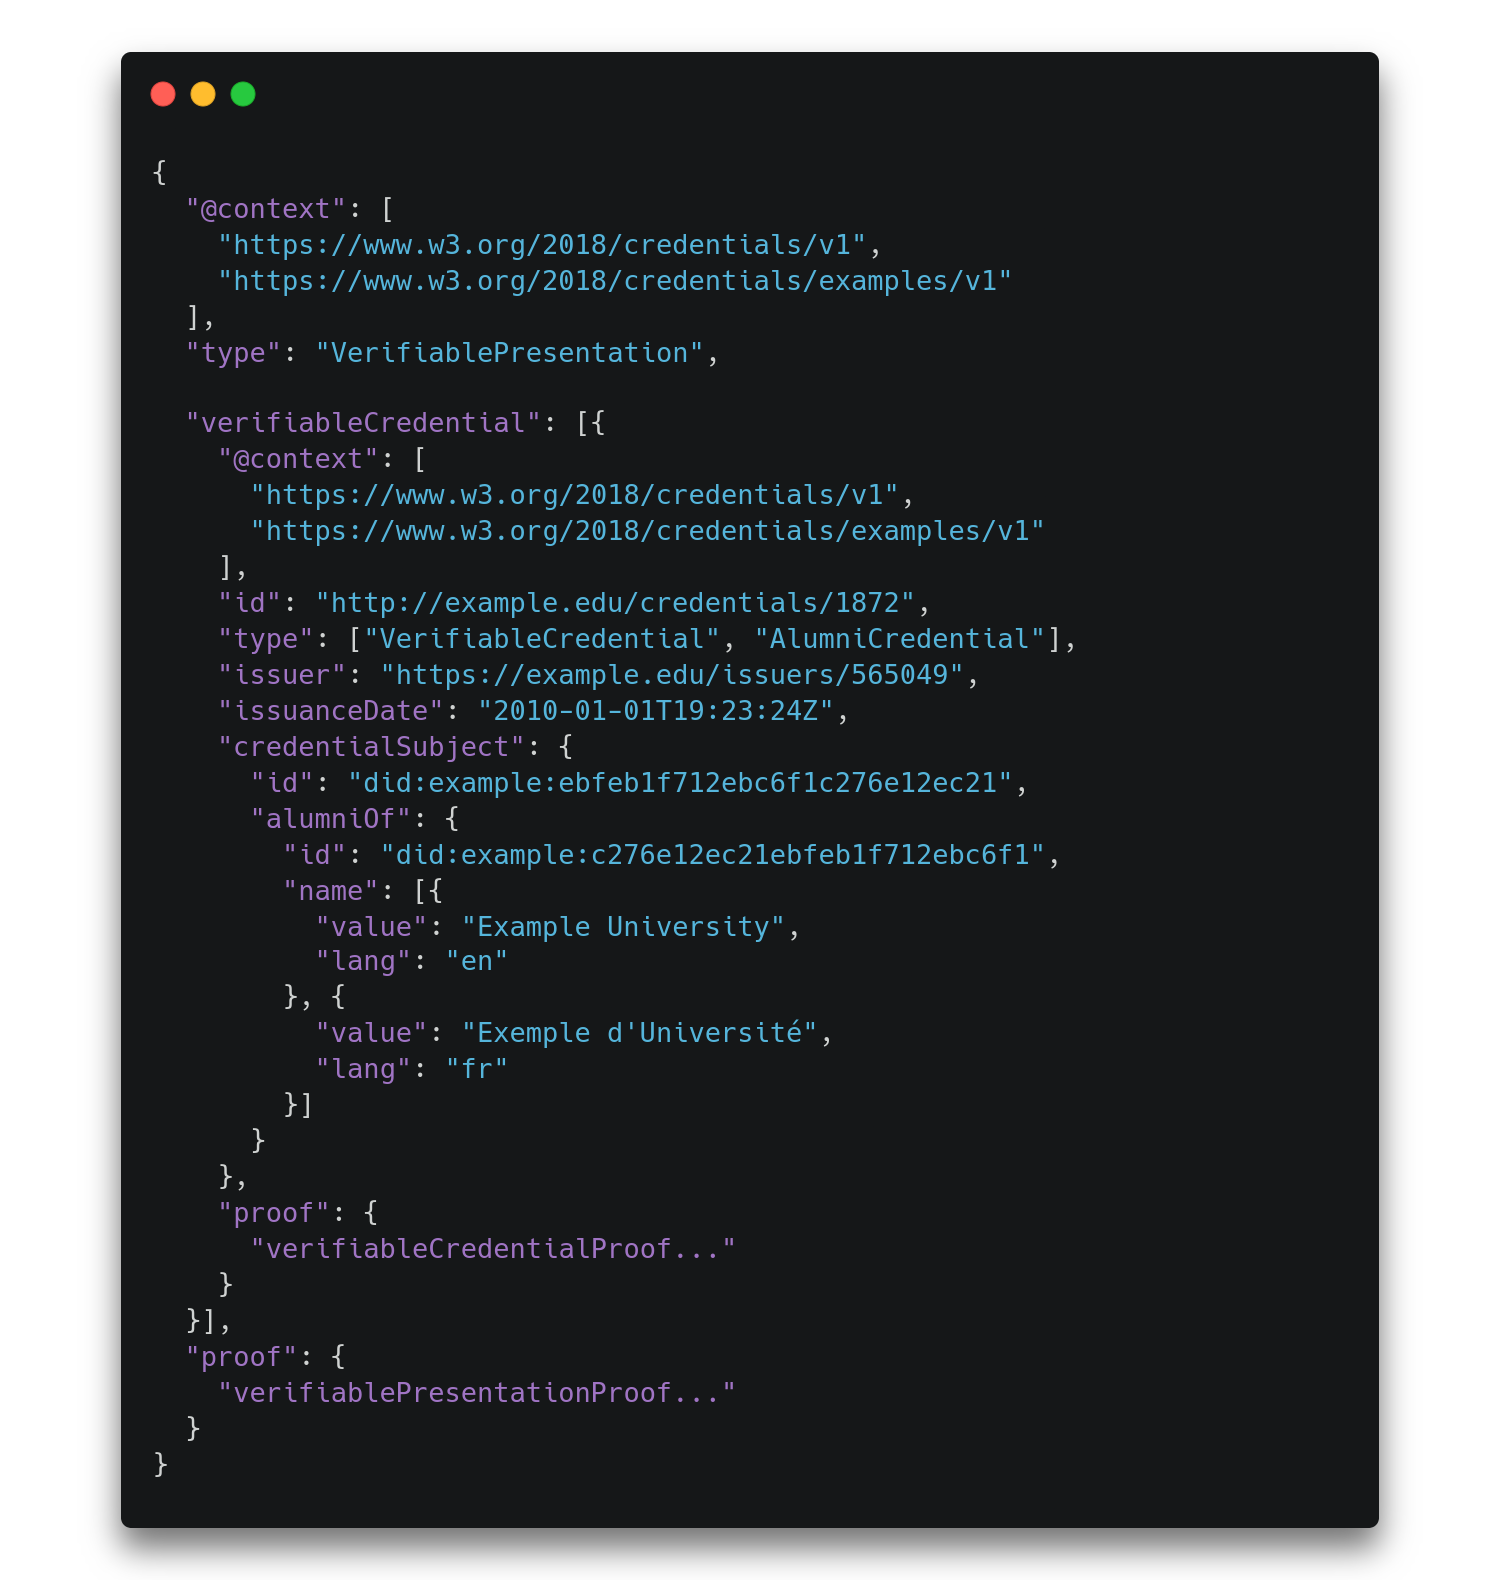
\includegraphics[scale=0.18]{chapter2/exampleVp.png}
    \captionof{figure}{Example of verifiable presentation (VP)}
\end{center}
The data in a presentation is often about the same subject but might have been issued by 
multiple issuers. The aggregation of this information typically expresses an aspect of 
a person, organization, or entity.

\subsubsection{Decentralized Identifier (DID)}
Decentralized identifiers are a new type of identifier that guarantees a verifiable, 
decentralized digital identity. A DID refers to any subject (e.g., a person, an 
organization, a data model, an abstract entity...).\\
DIDs are decoupled from centralized registries, identity providers, and certification 
authorities. Specifically, while other parties can be used to retrieve information 
about a DID, the design allows the controller of a DID to demonstrate control over it 
without requiring permission from other parties.
\begin{figure}[!htb]
    \begin{minipage}{0.48\textwidth}
      \centering
      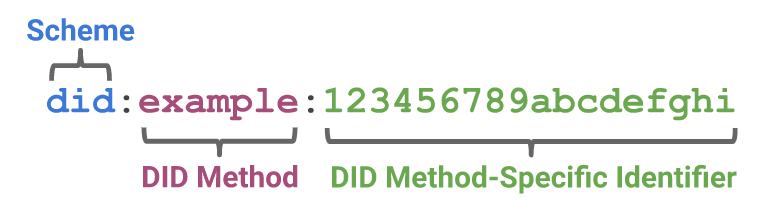
\includegraphics[width=1\linewidth]{chapter2/did1.png}
      \vspace{1.1cm}
      \caption{Example of a DID}
    \end{minipage}\hfill
    \begin{minipage}{0.48\textwidth}
      \centering
      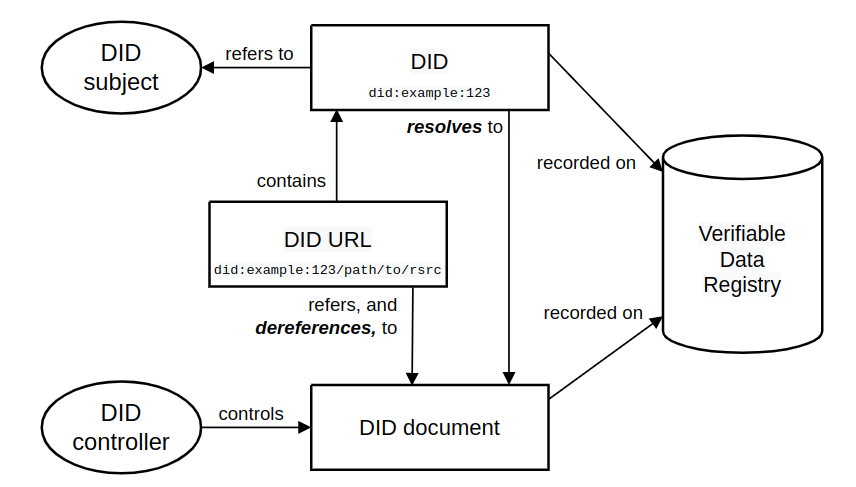
\includegraphics[width=1\linewidth]{chapter2/did2.png}
      \caption{DID architecture overview and basic components relationship}
    \end{minipage}
 \end{figure}
\begin{center}
    \vspace{-0.8cm}
    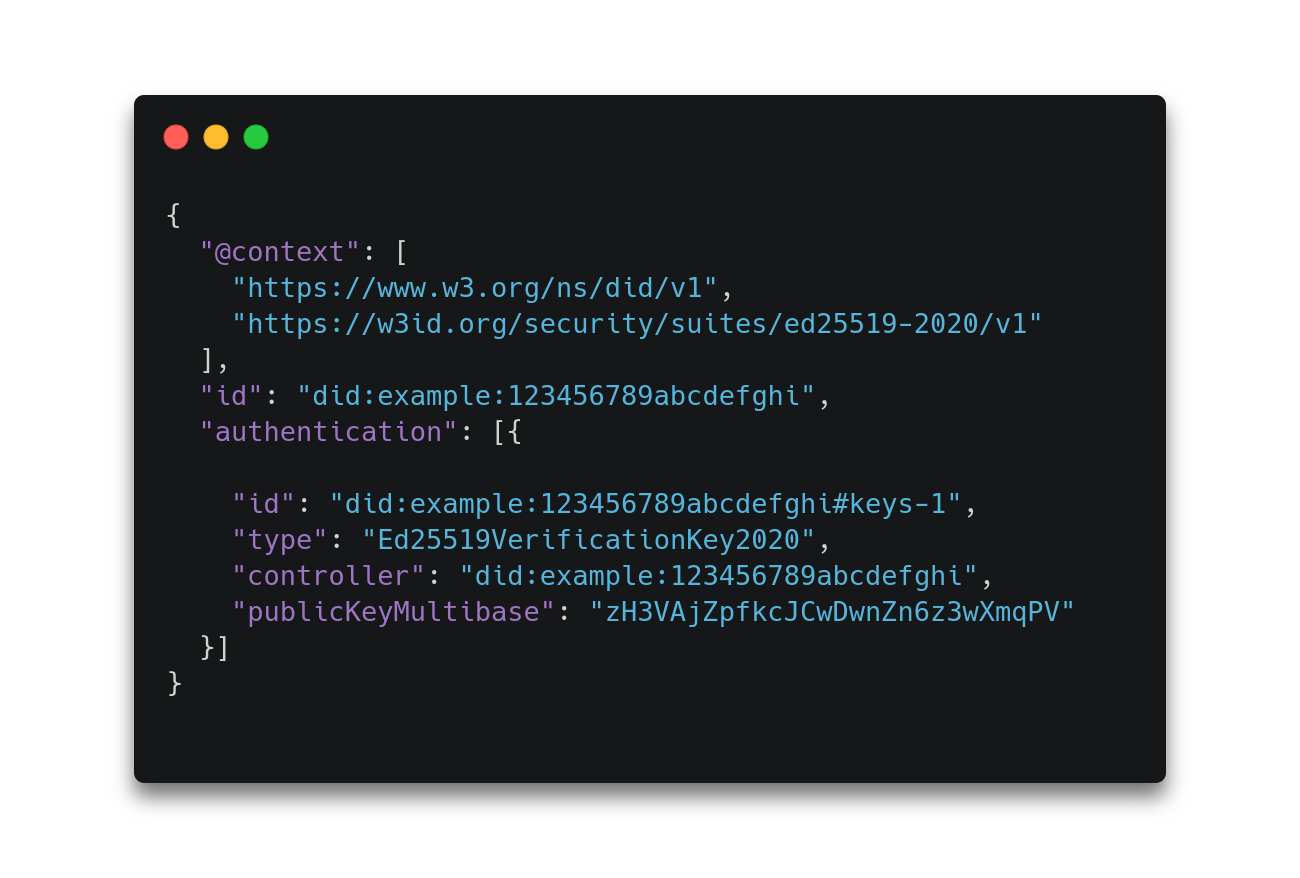
\includegraphics[scale=0.19]{chapter2/didDoc.png}
    \vspace{-0.4cm}
    \captionof{figure}{Example of DID document}
\end{center}
\vspace{0.5cm}
DIDs are Uniform Resource Identifiers (URIs) that associate a DID subject with a DID 
document that enables trusted interactions associated with that subject.
Each DID document may contain encrypted material, verification methods, or services, 
which provide a set of mechanisms that allow a DID controller to demonstrate control 
of the DID. Services enable trusted interactions associated with the subject of the 
DID. A DID may provide the means to return the DID subject itself if the DID subject 
is an information resource such as a data model.\\
A DID is a simple text string consisting of three parts: 1) the DID URI scheme 
identifier \footnote{The formal syntax of a decentralized identifier. The generic 
DID scheme begins with the prefix \textit{did:}.}, 2) the identifier for the DID method
\footnote{A definition of how a specific DID method scheme is implemented.}, and 3) 
the DID method-specific identifier.

\subsubsection{JavaScript Object Notation (JSON)}
\label{subsubsec:json}
The VC, VP and DID document code examples showed above are all in JSON.\\
The JSON is a lightweight data-interchange format. It is easy for humans to read and 
write, and for machines to parse and generate. It is based on a subset of the JavaScript
Programming Language Standard ECMA-262 3rd Edition - December 1999.\\
JSON is built on two structures:
\begin{itemize}
    \item A collection of name/value pairs. In various languages, this is realized as an 
    object, record, struct, dictionary, hash table, keyed list, or associative array.
    \item An ordered list of values. In most languages, this is realized as an array, 
    vector, list, or sequence.
\end{itemize}
These are universal data structures. Virtually all modern programming languages support 
them in one form or another. It makes sense that a data format that is interchangeable 
with programming languages also be based on these structures.
\subsection{Blockchain concepts}
Here we will introduce the main concepts of blockchain technology, essentials to 
understand the PoC development phase and some SDK features.
\subsubsection{Blockchain}
The blockchain is a shared, immutable database structured in the form of a chain of 
blocks, each of which contains a set of information. In essence, blockchains represent 
digital ledgers and perform different functions.
\begin{center}
    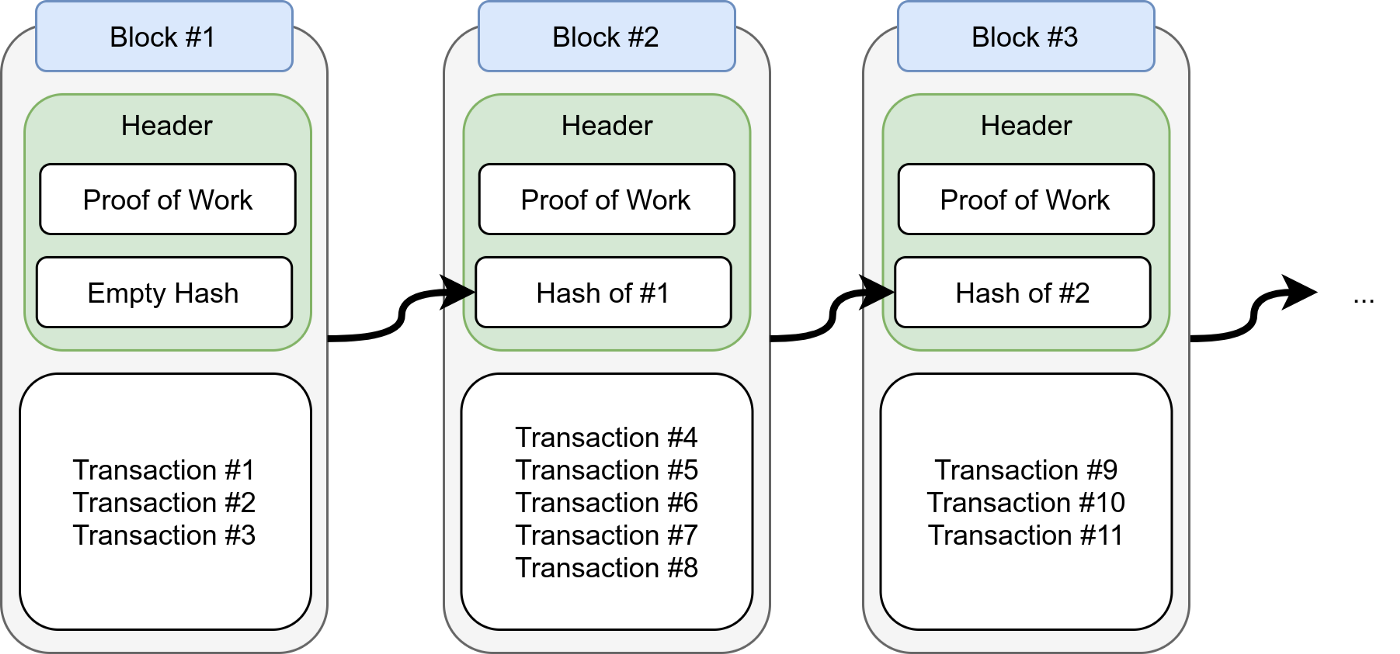
\includegraphics[scale=0.2]{chapter2/blockchain.png}
    \captionof{figure}{Simple blockchain visualization}
\end{center}
Physically it is composed of multiple \textbf{nodes}, i.e., computers that run the software 
(Client) of the blockchain. When a user wants to interact with the blockchain, he 
sends a \textbf{transaction} to one of the nodes. This transaction will then reach a pool with 
all the transactions in the pending state, and the nodes that are dealing with the 
consensus part will take care of updating the state of the blockchain by inserting 
several transactions (meeting certain conditions) within the new \textbf{block} that will
be added to the chain.\\
Its main features are data digitalization, decentralization, disintermediation, 
transfer traceability and programmability, transparency/verifiability, and immutability.
\subsubsection{Permissionless and permissioned blockchains}
We can divide blockchains into two main categories: permissionless and permissioned.
This division is based on the access to the network.
\begin{itemize}
    \item \textbf{Permissionless blockchains} are the most popular model. As its name implies, these 
    networks allow access to anyone and are decentralized and public. Consequently, 
    everyone can run a node or connect to the blockchain.\\
    This accessibility implies a trade-off on speed; these networks are often slower than 
    their permissioned counterparts, with fewer members, and transactions are validated by 
    everyone running a connected node. The primary consensus mechanisms are Proof-of-Work 
    (PoW) and Proof-of-Stake (PoS) \footnote{PoW involves hashing (mining) power, PoS voting 
    (using blockchain coins) power, through validator nodes.}.\\
    What is of most interest in this scenario is that in a permissionless blockchain, 
    everyone can interact, and data is public, so \textbf{preserving privacy becomes difficult}.
    \item \textbf{Permissioned blockchains} are private networks that require permission to
    join. They are usually run by a single organization or a consortium of organizations.\\
    The main advantage of permissioned blockchains is speed. They are faster than
    permissionless blockchains because they have fewer members and transactions are
    validated by a smaller number of nodes. The main consensus mechanisms are Raft and 
    Practical Byzantine Fault Tolerance (PBFT).\\
    The main peculiarity of permissioned blockchains is that they are not decentralized
    and are not public. This means that only a limited number of people can interact with
    the blockchain, and data is not public, so \textbf{privacy can be preserved}.
\end{itemize}

\subsubsection{Ethereum}
Ethereum is a permissionless blockchain, i.e., open to anyone who wants to interact 
with it: the trade-off is the introduction of fees, to be paid every time anyone wants 
to change the state of the Ethereum Virtual Machine (EVM), to mitigate the problems 
that the permissionless factor introduces (e.g., transaction spam). In the read-only 
case, no fee needs to be paid. Anyone can then view what is happening in the blockchain 
and, more importantly, use it. To do so, a user has to generate a \textbf{wallet} (i.e.,
an address in the blockchain), transfer some funds to it from outside \footnote{Usually
from a centralized exchange, where cryptoc-urrencies can be traded for fiat currencies
like EUR or USD, or from another blockchain.} so that fees can be paid, and start 
interacting with the decentralized applications that are already developed or transfer 
funds to other wallets. In fact, one of the main features of Ethereum is \textbf{smart 
contracts}: they are programs that run on the Ethereum blockchain. They are a collection 
of code (functions) and data (state) that resides at a specific address on the 
Ethereum blockchain.
\subsubsection{Hyperledger}
Hyperledger Foundation is a nonprofit organization that combines all the resources and 
infrastructure needed to ensure thriving and stable ecosystems around open-source 
software blockchain projects.\\
Hyperledger Foundation staff are part of the larger \textbf{Linux Foundation} team with
years of experience providing management services for programs for open-source projects.
\subsubsection{Hyperledger Besu}
Hyperledger Besu is an Ethereum client designed to be enterprise-friendly for use cases 
of public and private permissioned networks, which require secure transaction processing
and high performance.\\
The Besu blockchain, therefore, is EVM compatible: from the perspective of developers 
and users, interaction with it will be very similar to interaction with Ethereum. It 
places particular emphasis, however, on \textbf{privacy and permissioning} features; in fact, 
only those who are authorized (i.e., those who own a connected node) can interact with 
the system, which is the primary difference from Ethereum.
\begin{figure}[!htb]
    \begin{minipage}{0.48\textwidth}
        \centering
        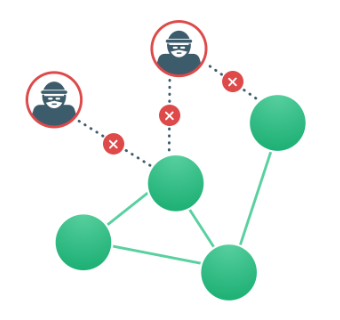
\includegraphics[width=.77\linewidth]{chapter2/privacyEsterno.png}
        \caption{Only allowed users can participate in the network}
    \end{minipage}\hfill
    \begin{minipage}{0.48\textwidth}
        \centering
        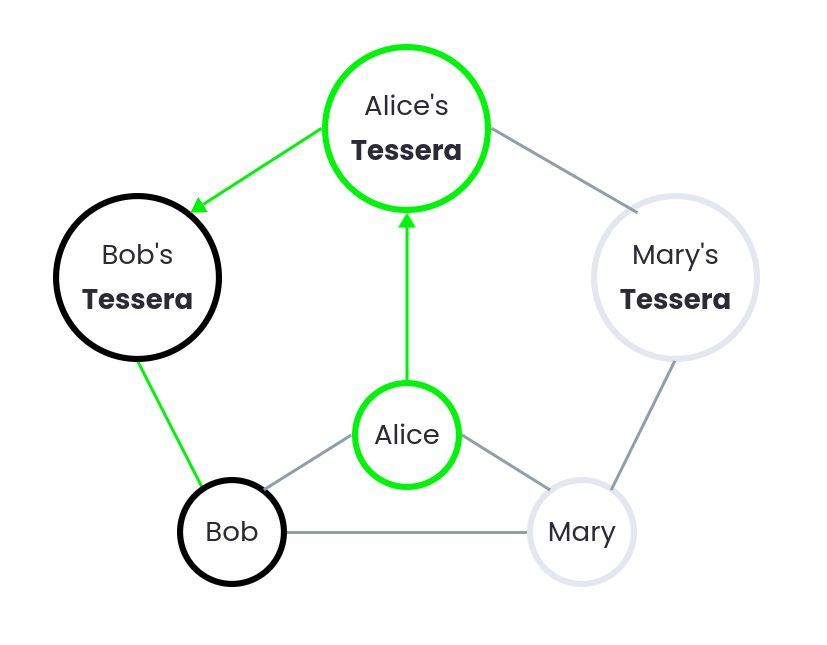
\includegraphics[width=1\linewidth]{chapter2/privacyInterno.png}
        \caption{Mary cannot see the private transaction sent from Alice to Bob}
    \end{minipage}
\end{figure}
\begin{figure}[!htb]
    \begin{minipage}{0.48\textwidth}
        \centering
        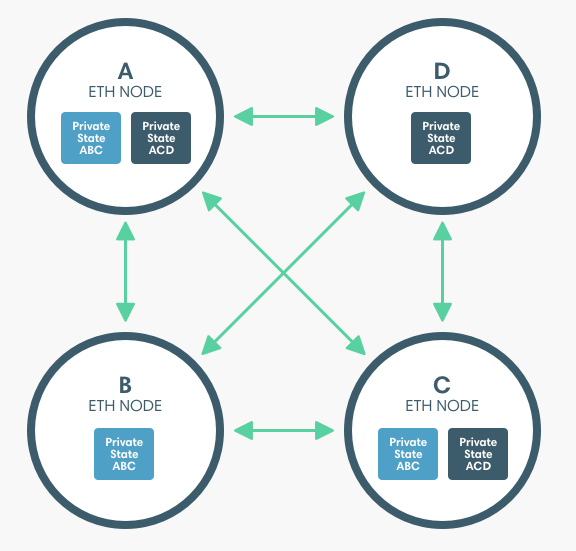
\includegraphics[width=.77\linewidth]{chapter2/privacyGroups.png}
        \caption{Restricted visibility of two Privacy Groups (light blue and blue)}
    \end{minipage}\hfill
    \begin{minipage}{0.48\textwidth}
        \centering
        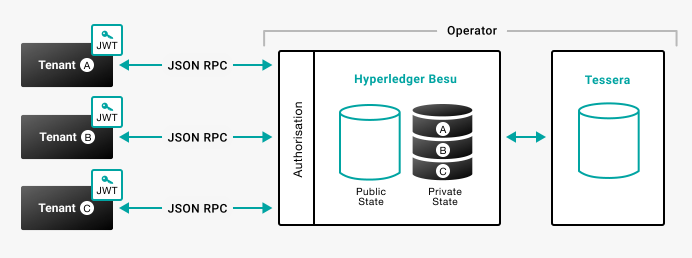
\includegraphics[width=1\linewidth]{chapter2/multiTenant.png}
        \caption{Besu and Tessera pair nodes administrator can give access to other Tenants, i.e., users.}
    \end{minipage}
\end{figure}\\
Privacy is enabled both externally to the network and internally: through private 
transactions, not all nodes can access certain information, and nodes that want to 
take advantage of private transactions must have an associated \textbf{Tessera} node, which 
will take care of the cryptographic part.\\
Even \textbf{Privacy Groups} can be created: those who do not belong to the group cannot access 
particular data. In addition, another interesting feature is that of Multi-Tenant 
management: multiple participants can use the same Besu and Tessera node through a 
dedicated user system.

\subsubsection{Hyperledger Fabric}
Hyperledger Fabric is an enterprise-grade, proven, and open distributed ledger 
platform (DLT). It provides advanced privacy controls so that only the shareable 
data is transmitted among network participants, known as "authorized".\\
It offers a modular architecture that makes available components (mechanism for 
consensus, services for joining and managing blockchain members) that can be activated
within a blockchain with plug-and-play logic. It can be said to be very similar to 
Besu (also a permissioned and privacy-oriented), with the big difference being that 
it is not EVM compatible so the smart contracts will be written in languages such as 
Java and Go instead of Solidity.
\subsection{Libraries and Stack involved}
After analyzing all the necessary pre-concepts, we can now introduce the last ones:
EBSI, which can be used as VDR, and walt.id, the software suite that includes the SSI 
Kit.
\subsubsection{EBSI}
European Blockchain Services Infrastructure (EBSI) is a service infrastructure for 
managing European citizens' identity and education credentials. These use cases aim 
to facilitate the mobility of students, young professionals, and entrepreneurs, as 
well as ensure and verify the authenticity of digital information in different 
sectors.
\begin{center}
    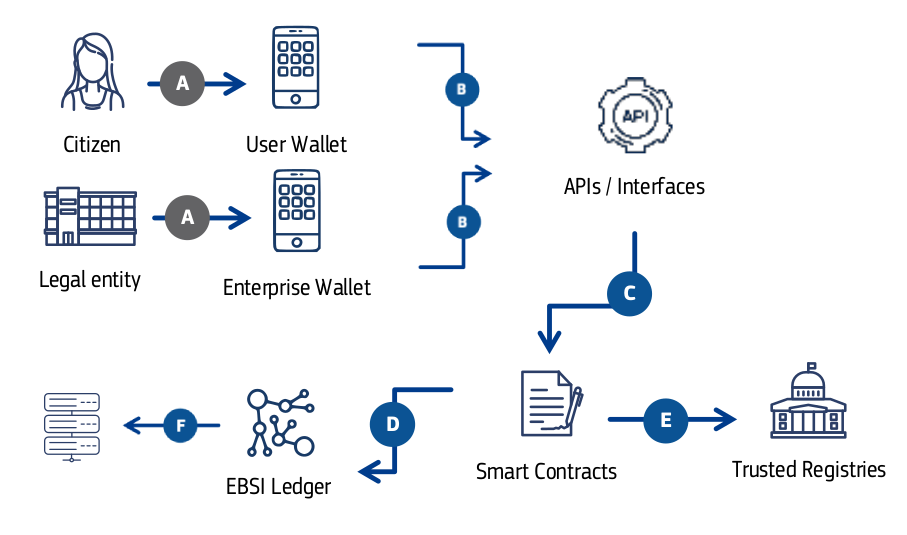
\includegraphics[scale=0.27]{chapter2/ebsiflow.png}
    \captionof{figure}{EBSI interaction flow}
\end{center}
Its structure is rather complex, consisting of two essential layers: the bottom layer 
is made up of EBSI's blockchain, which holds all the credentials and smart contracts 
with which one can interact with them, while the upper layer by a microservices 
architecture and Application Programming Interface (API), which interface with the 
blockchain. In practice, to talk to the EBSI blockchain (if you do not have a node), 
you must interface through the microservices architecture and API. The blockchains
used by EBSI are Hyperledger Fabric and Hyperledger Besu.\\
Finally, in the blockchain are already deployed a series of smart contracts, serving 
as a registry for DIDs (and DID documents) and for trusted applications, issuers, 
ledgers, and policies.
\subsubsection{walt.id SSI Kit}
The walt.id software suite, an open-source project developed by a European team, 
consists of a set of kits that allows us to add SSI functionalities to our product. 
Specifically, by leveraging the SSI Kit, it will be possible to generate encrypted 
keys, register and resolve DIDs, create, issue, submit and verify VCs, and much more. 
This kit can be used via Command Line Interface (CLI) or REST API. Currently, the 
kit supports \texttt{did:key}, \texttt{did:web}, and \texttt{did:ebsi} methods (the 
latter allows us to talk to the EBSI blockchain). Since, by default, it dialogues with 
other APIs (e.g., EBSI's API), if we wanted to register, for example, a DID in a 
mainnet that has not yet been registered, such as Sovrin, we would need to add the 
\texttt{did:sov} method to the list of supported methods, also implementing the 
dialogue with Sovrin's API. Doing this would require a new module development, 
integrating it with the SSI Kit, and developing something similar to what has been 
done for EBSI, although the complexity is unknown.
% /*//////////////////////////////////////////////////////////////
%                        STATE OF THE ART
% //////////////////////////////////////////////////////////////*/
\section{State of the art}
Taking back the purpose of this paper, we want to build a hybrid solution, merging SSI 
with blockchain smart contracts. Currently, within SSI, most blockchains are used only 
as VDR (so to store DIDs, VC verification policies, schemas...).\\
The final software (PoC) has to leverage a kit to offer SSI functionalities (SDK) and 
combine these with blockchain features to automate verifications and possibly 
facilitate certain issuing cases (smart contract suite).\\
That said, we can now illustrate what already exists and what has to be crafted.
\subsection{Complete solution}
"Complete solution" means a software that already merges an SSI SDK with a smart 
contract suite. Unfortunately, during the first two weeks of research and situation 
study, we did not find anything already built, probably because of the technologies 
involved novelty.\\
As a result, we must find existent SDKs and smart contract standards to build the 
desired solution and, if not, build everything from scratch.
\subsection{SSI Kits}
As already stated and introduced, SSI Kit by walt.id is a Swiss Army knife for SSI 
primitives. However, it has been chosen after analyzing other existing 
solutions.\\
Initially, we were looking for a kit that provides multichain support (i.e., the 
possibility to interact with more DIDs across multiple blockchains). 
Unfortunately, an equivalent of the SSI Kit with multiple chains support does not 
exist, and every other found kit supports at most one blockchain. The Decentralized 
Identity Foundation (DIF) develops the most interoperable tools we found in the SSI
scope: Universal Resolver and Universal Registrar.\\
We now describe all the solutions we found and specify why we choose the SSI Kit by 
walt.id.
\vspace{0.35cm}\\
Firstly, all the existing kits support the two main DID methods:
\begin{itemize}
    \item \texttt{\textbf{did:key}}: a non-registry based method that generates a DID
    from a cryptographic key. It is the simplest method;
    \item \texttt{\textbf{did:web}}: a method that generates a DID that enables the 
    use of an existing web domain as identifier.
\end{itemize}
Other than SSI Kit by walt.id, we found two SDKs developed by MATTR and Veramo Labs.
In this table, we will outline the kit, which DID method is supported other than the 
two discussed, the documentation status, and whether the kit is free to use.
\renewcommand{\arraystretch}{1.75}
\vspace{0.1cm}\\
\begin{table}[h]
    \begin{center}
        \rowcolors{2}{lighter-grayer}{white}
        \begin{tabular}{ |c|c|c|c|c| } 
            \hline
            \rowcolor{lighter-gray}
            \textbf{SSI Kit} & \textbf{DID method} & \textbf{Documentation}
             & \textbf{Free to use} & \textbf{Support}\\
            \hline
            walt.id & did:ebsi & Improvable \tablefootnote{Improvable: not everything
            is documented so we must read the source code or contact the team} & Yes & 
            Team, Slack\\ 
            MATTR & did:ion \tablefootnote{DID method to interact with ION, a Bitcoin 
            sidechain} & Good & No & E-mail\\ 
            Veramo & did:ethr \tablefootnote{DID method to interact with Ethereum} & 
            Improvable & Yes & Discord\\ 
            \hline
        \end{tabular}
        \vspace{0.2cm}
        \caption{Analyzed kits}
    \end{center}
\end{table}
\vspace{-0.5cm}\\
To summarize:
\begin{itemize}
    \item \textbf{MATTR} SDK adds support for \texttt{did:ion} method. Its biggest flaw is 
    the lack of support from the team: the only method to reach them is by sending an e-mail. 
    In addition, the kit is not free to use.
    \item \textbf{Veramo} SDK supports the \texttt{did:eth} method. We need to join the
    Discord server (not so active) to ask for support, the SDK is free, but the 
    documentation could be improved.
    \item \textbf{walt.id} SSI Kit adds support for the EBSI blockchain. It is free to 
    use, and the documentation is improvable, but as the kit is in development, the 
    team is very active in the Slack channel (also, Monokee had direct contact with the
    walt.id team).
\end{itemize}
After the research, we choose walt.id SSI Kit, mainly because the kit offered more 
functionalities and was more customizable. Additionally, it supported EBSI, which was 
a good "nice-to-have" for Monokee, as in contact with the University of Naples 
Federico II to build a project interacting with the European blockchain.\\
Finally, the team was very active and chose to support us in developing the SDK for 
walt.id SSI Kit.

\subsection{Smart contract suites}
Regarding the use of smart contracts in the SSI environment, we first need to know how they 
can be used.\\
The roles they can assume, following the SSI model, are two: issuer and verifier (holder 
would not make much sense). The role we already know they can assume is a register of DID 
and events like verification or revocation.
\vspace{0.3cm}\\
Let us now try to think about what should a smart contract need in order to be an issuer or 
a verifier:
\begin{itemize}
    \item \textbf{Issuer}: he has to be able to produce a signature that confirms who is 
    issuing owns the DID (to certify his identity), other than to generate a VC.
    This has to be made with the private key of that DID, and everyone can verify the signer's 
    identity with the public key. After a discussion with the Monokee team, we decided to 
    avoid implementing this unless we find something already done.
    \item \textbf{Verifier}: he has to be able to verify a VC, which means he has to take it 
    in input and verify it using the verification method described in the appropriate field. 
    Also, to enhance trust, it should sign the verification result with the private key of 
    its DID. Again, these functions could be hard to implement inside a smart contract, so we 
    came to the same conclusion.
\end{itemize}
Our research uncovered two libraries: one for the leading and most used patterns and one 
for the SSI features.\\
The first one is an extensive collection of patterns and security standards developed by 
\textbf{OpenZeppelin}. It ranges from the simplest things, such as a counter standard contract, to 
the most complex, such as Ethereum Request for Comments (ERC) implementations (ERC-20 is 
one of the most famous, and it is the standard for Ethereum fungible tokens)
For example, we will use the ERC-721 implementation (Non-Fungible Tokens, or NFTs) to 
implement one of the use cases.\\
The second one is a suite of smart contracts that aims to bring SSI on-chain. It is called 
\textbf{Verite} and is being developed by Centre (to give a background, Centre is the company
that developed USDC, one of the leading stablecoins in the cryptocurrency market).
As it stands, the library only contains a smart contract that serves as a verification 
results registry, and we decided to take it and adapt it to our purposes.
\vspace{0.3cm}\\
Since, during our research, we did not find an implementation of on-chain issuer or verifier 
agents, we decided to re-use already existing smart contract libraries and build some simple
auxiliary smart contracts we needed in order to implement on-chain registries to at least 
make some actions more immediate (like verifications and revocations).
